% Preamble
\documentclass[onecolumn, twocolappendix]{aastex631}
%\documentclass[twocolumn]{aastex631}
\usepackage{natbib}
\usepackage{latexsym}
\usepackage{graphicx}
\usepackage{epsfig}
\usepackage{amssymb}
\usepackage{amsmath}
\usepackage{epstopdf}
\usepackage{hyperref}
\usepackage{xcolor}

%%%% Custom commands
\newcommand{\yL}{\ensuremath{\mathcal{Y}_{\rm{L}}}}
\newcommand{\yS}{\ensuremath{\mathcal{Y}_{\rm{S}}}}
\newcommand{\justgrad}{\ensuremath{\nabla}}
\newcommand{\gradrad}{\ensuremath{\nabla_{\rm{rad}}}}
\newcommand{\gradad}{\ensuremath{\nabla_{\rm{ad}}}}
\newcommand{\gradC}{\ensuremath{\nabla_{\mathrm{C}}}}
\newcommand{\gradmu}{\ensuremath{\nabla_{\mu}}}
\newcommand{\gradL}{\ensuremath{\nabla_{\mathrm{L}}}}
\newcommand{\gradT}{\ensuremath{\nabla_{\mathrm{T}}}}
\newcommand{\Ro}{\ensuremath{\mathrm{R}_{0}}}
\newcommand{\delp}{\ensuremath{\delta_{\rm{p}}}}
\newcommand{\Fbot}{\ensuremath{F_{\rm{bot}}}}
\newcommand{\Ftot}{\ensuremath{F_{\rm{tot}}}}
\newcommand{\Frad}{\ensuremath{F_{\rm{rad}}}}
\newcommand{\Fconv}{\ensuremath{F_{\rm{conv}}}}
\newcommand{\Fcz}{\ensuremath{F_{\rm{cz}}}}
\newcommand{\mP}{\ensuremath{\mathcal{P}}}
\newcommand{\mD}{\ensuremath{\mathcal{D}}}
\newcommand{\dP}{\ensuremath{\delta_{\rm{p}}}}
\newcommand{\Lcz}{\ensuremath{L_{\rm{CZ}}}}
\newcommand{\mR}{\ensuremath{\mathcal{R}}}
\newcommand{\mS}{\ensuremath{\mathcal{S}}}
\newcommand\Pran{\ensuremath{\mathrm{Pr}}}
\newcommand{\brunt}{{Brunt-V\"{a}is\"{a}l\"{a}}}

\newcommand{\angles}[1]{\langle #1 \rangle}
\newcommand{\pd}[1]{\partial_{#1}}
\renewcommand{\vec}[1]{\boldsymbol{#1}}
\newcommand{\M}[1]{\mathbf{#1}}
\renewcommand{\dot}{\vec{\cdot}}
\renewcommand{\bar}[1]{\overline{#1}}
\newcommand{\grad}{\vec{\nabla}}
\newcommand{\cross}{\vec{\times}}
\newcommand{\laplacian}{\nabla^2}

\newcommand{\editone}[1]{\textcolor{orange}{#1}}

%%%% Journal preamble
\received{April 1, 2022}
\revised{April 1, 2022}
\accepted{???}
%\published{April 1, 2022}
\submitjournal{The Journal of Universal Rejection}

\shorttitle{Moosinesq Convection}
\shortauthors{Anders et al}

\begin{document}

%%%% Title and Abstract
\title{Moosinesq Convection in the Cores of Moosive Stars}
\author[0000-0002-3433-4733]{Evan H. Anders}
\affiliation{CIERA, Northwestern University, Evanston IL 60201, USA}
\author[0000-0002-4791-6724]{Evan B. Bauer}
\affiliation{Center for Astrophysics $\vert$ Harvard \& Smithsonian, 60 Garden St., Cambridge, MA 02138, USA}
\author[0000-0001-5048-9973]{Adam S. Jermyn}
\affiliation{Center for Computational Astrophysics, Flatiron Institute, New York, NY 10010, USA}
\author[0000-0001-8935-219X]{Benjamin P. Brown}
\affiliation{Department Astrophysical and Planetary Sciences \& LASP, University of Colorado, Boulder, CO 80309, USA}
\author[0000-0003-1651-9141]{Eric W. Hester}
\affiliation{Department of Mathematics, The University of California, Los Angeles, 520 Portola Plaza 90024, California, United States of America}
\author{Mindy Wilkinson}
\affiliation{Primum Terrae LLC, Boulder, CO 80302, USA}
\author[0000-0003-1012-3031]{Jared A. Goldberg}
\affiliation{Department of Physics, University of California, Santa Barbara, CA 93106, USA}
\author[0000-0002-4472-8517]{Samuel J. Van Kooten}
\affiliation{Southwest Research Institute, Boulder CO 80302, USA}
\author[0000-0003-0256-9295]{Tania Varesano}
\affiliation{Grenoble Institute of Technology, Grenoble, France}
\affiliation{Southwest Research Institute, Boulder CO 80302, USA}
\author[0000-0002-7635-9728]{Daniel Lecoanet}
\affiliation{CIERA, Northwestern University, Evanston IL 60201, USA}
\affiliation{Department of Engineering Sciences and Applied Mathematics, Northwestern University, Evanston IL 60208, USA}

\correspondingauthor{Evan H. Anders}
\email{evan.anders@northwestern.edu}

\begin{abstract}
    Stars with masses $\gtrsim 4 \times 10^{27}M_{\rm{moose}} \approx 1.1 M_\odot$ have core convection zones during their time on the main sequence.
    In these \emph{moosive stars}, convection introduces many uncertainties in stellar modeling.
    In this Letter, we build upon the Boussinesq approximation to present the first-ever simulations of \emph{Moosinesq convection}, which captures the complex geometric structure of the convection zones of these stars.
    These flows are bounded in a manner informed by the majestic terrestrial \emph{Alces alces} (moose) and could have important consequences for the evolution of these stars.
    We find that Moosinesq convection results in very interesting flow morphologies and rapid heat transfer, and posit this as a mechanism of biomechanical thermoregulation.
\end{abstract}
\keywords{Moose, Meese, Mice}

%%%% Body of paper
\section{Introduction}
\label{sec:introduction}

Convection is important in all sorts of natural systems\footnote{Trust us, we're experts}.
In particular, most stars have convection zones.
This can be determined by looking at the Sun\footnote{Please do not look at the Sun.} or by running 1D stellar evolution models.
It is crucial that we gain a better understanding of convection since it is such a ubiquitous and poorly understood process in astrophysics\footnote{The financial wellfare of many of the authors depends on you agreeing with this statement.}.

Convective motions are three-dimensional, so many modern experiments use multi-dimensional fluid dynamical simulations.
However, modern computational resources are too limited to time-evolve the Navier-Stokes equations in their most complex form \citep{landau}, a form required by all of the important physics present in stars \citep{Paxton2011, Paxton2013, Paxton2015, Paxton2018, Paxton2019}.
As a result, numericists make simplifying assumptions to create tractable experiments, for example by simplifying the geometry or the equations.
The most widely-used simplified set of equations employs the \emph{Boussinesq approximation}\footnote{Or the ``incompressible except for when it's not'' approximation, though this term has not caught on in the literature.} \citep{spiegel_veronis_1960}, and it has been used in thousands of studies \citep[see e.g.,][]{ahlers_etal_2009}.

In this Letter, we present the first ever simulations that use an oft-overlooked fluid approximation: the \emph{Moosinesq} approximation.
The Moosinesq and Boussinesq approximations are identical in every way, except convection inside of a moose (\emph{Alces alces}) can only be studied under the Moosinesq approximation.
This approximation is suitable for describing the active and dynamic inner lives and environments (both physical and mental; see \citealp{Gibson2015}) of the moose.
The moose is a large mammal indigenous to North America and Europe and can have a mass of up to $M_\mathrm{moose}\equiv 550$~kg and a vertical length scale of up to $L_\mathrm{moose} \equiv 2$~m \citep{CPWmoose}.
The word ``moose'' is seen in observations to be both singular and plural, a fact that has long eluded explanation by even the most talented theorists.
Our study is not the first time that moose have prompted significant scientific or technological development \citep[see, e.g.,][]{Handel2009}.
For a brief taste of the rich historical interactions between humanity and moose, we refer the reader to appendix~\ref{app:history}.

While Moosinesq convection has many\footnote{\emph{many}} applications in the terrestrial context, the authors of this Letter are mostly astrophysicists.
Therefore we focus on the application of this approximation to \emph{moosive stars}, that is, stars with masses $M \gtrsim 4\times 10^{27} \; M_\mathrm{moose}$ (or $1.1 \; M_\odot$) which have convective cores while on the main sequence.
In section \ref{sec:methods}, we describe the Moosinesq equations and our numerical methods.
In section \ref{sec:results}, we demonstrate the nature of flows in two-dimensional Moosinesq convection.
Finally, in section \ref{sec:conclusions}, we discuss applications of Moosinesq convection to stars, human society, and beyond.


\section{Numerical methods}
\label{sec:methods}

\begin{figure*}[t!]
\centering
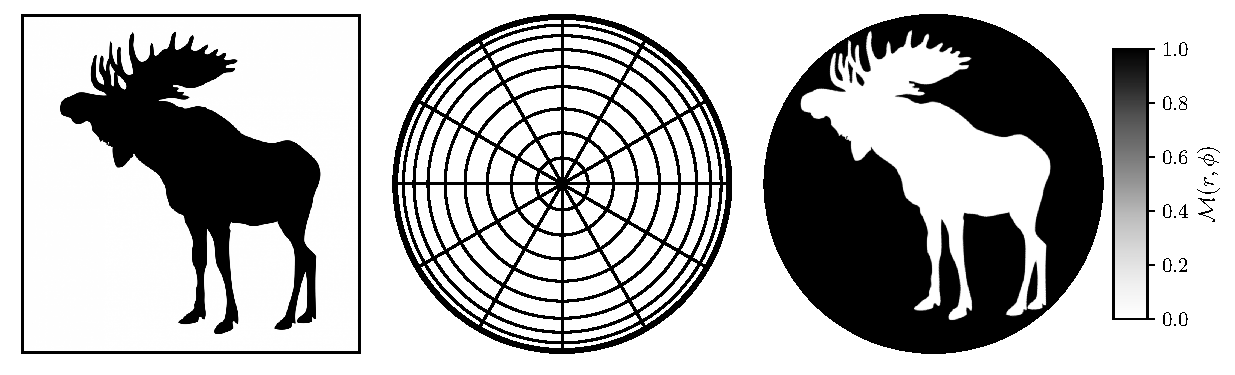
\includegraphics[width=\textwidth]{paper_figure01.pdf}
    \caption{ 
        (Left) A public-domain silhouette of a moose.
        (Middle) A sparse representation of the polar-coordinate grid on which we represent fields in our simulation.
        (Right) The Moosinesq mask $\mathcal{M}$ felt by our equations; fluid motions are damped where $\mathcal{M} > 0$.
        \label{fig:methods}
    }
\end{figure*}

Words about Fig.~\ref{fig:methods} (left)\footnote{Available online at \url{https://www.publicdomainpictures.net/en/view-image.php?image=317077&picture=moose}.}.


\section{Results}
\label{sec:results}

We display the majesty of Moosinesq convection in Fig.~\ref{fig:dynamics}.
We visualize the temperature field $T$, so red is warm fluid that buoyantly rises, and blue is cold fluid that buoyantly falls.
Plotted over the temperature field is the mask $\mathcal{M}$, which is fully transparent when it is zero and which is a low-opacity white when $\mathcal{M} = 1$.
This allows us to show that, indeed, there are no appreciable motions outside of the moose and the mask is working properly.

The moose is filled with interesting dynamics\footnote{Likely due to a recent, delicious meal.}.
The legs largely serve as thin, tall ``tunnels'' which are filled with Von K\'{a}rm\'{a}n vortices and which connect the hot moose feet to its neutrally-buoyant body.
Cold fluid parcels from the body have managed to mix down one leg, and the moose would probably benefit from having that leg wrapped in a warm cloth or heat pack.
The body of the moose exhibits dynamics familiar from classical 2D Rayleigh-B\`{e}nard convection.
Hot and cold fluid swirl together, forming many vortices which eventually mix.
Aside from the legs, the antlers are the most interesting part of the moose.
Vortices of relatively hot fluid establish themselves there and remain for a few convective overturn times.
Then, violent flows from the moose's body disrupt those vortices with fresh, hot fluid and this process repeats itself.
Occasionally some of this hot fluid rises into the tips of the moose's antlers, which explains how moose grow antlers.

\begin{figure*}[tp!]
\centering
    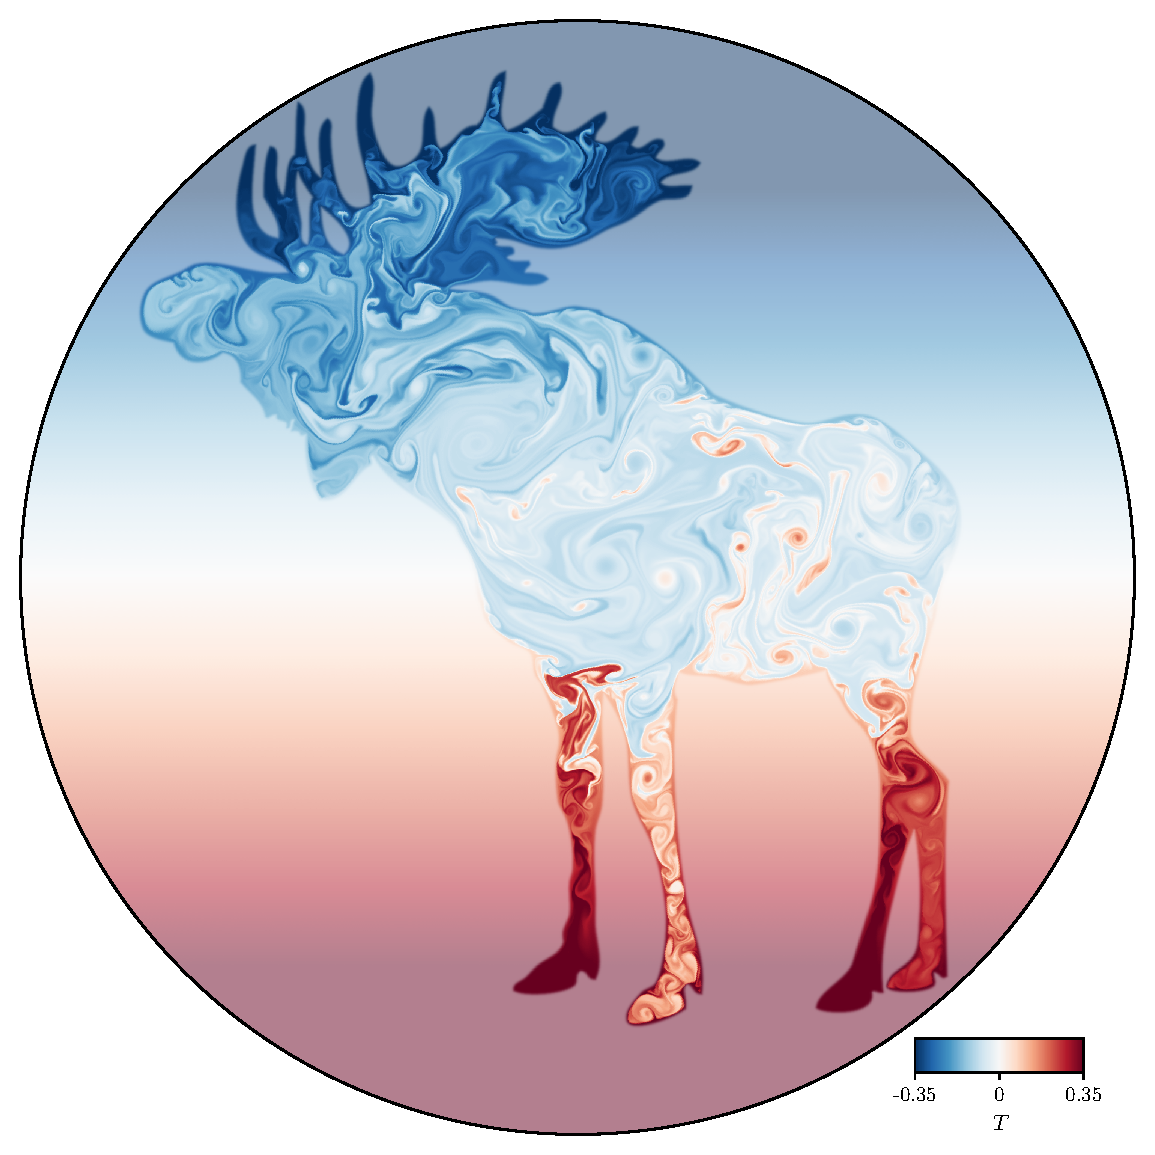
\includegraphics[width=\textwidth]{paper_figure02.pdf}
\caption{ 
    Here we visualize the temperature field in our simulation, where red is hot and buoyantly rises while blue is cold and buoyantly falls.
    We furthermore overplot the mask $\mathcal{M}$ on top of the temperature field in white with a low opacity; this does not affect the flow visualization within the moose but makes the region outside of the moose appear lighter in color.
    We do this to demonstrate that indeed, the flows are restricted to the area within $\mathcal{M}$ and therefore within the moose, as we expected.
    We encourage the reader to particularly note the beauty and power of the moose.
    A video version of this figure is available online at TODO.
\label{fig:dynamics}
}
\end{figure*}

Now that we have examined the dynamics in Moosinesq convection in some detail, we turn our attention towards its astrophysical applications.
\citet{kaiser_etal_2020} note that ``massive [sic] stars'' are sensitive to ``the details of their complex convective history''.
We agree.
When considering convective uncertainties in \emph{moosive} stars, previous authors have ignored the complex dynamics displayed in Fig.~\ref{fig:moosive_stars}.
That is, the cores of these stars are filled with Moosinesq convection, which can have important consequences for moosive stellar evolution.
it is unclear at this time how the complex flow morphologies associated with Moosinesq convection would affect e.g., the magnetic fields, chemical profiles, and lifetimes of these stars.
We leave these important considerations to future work.

\begin{figure*}[t!]
\centering
    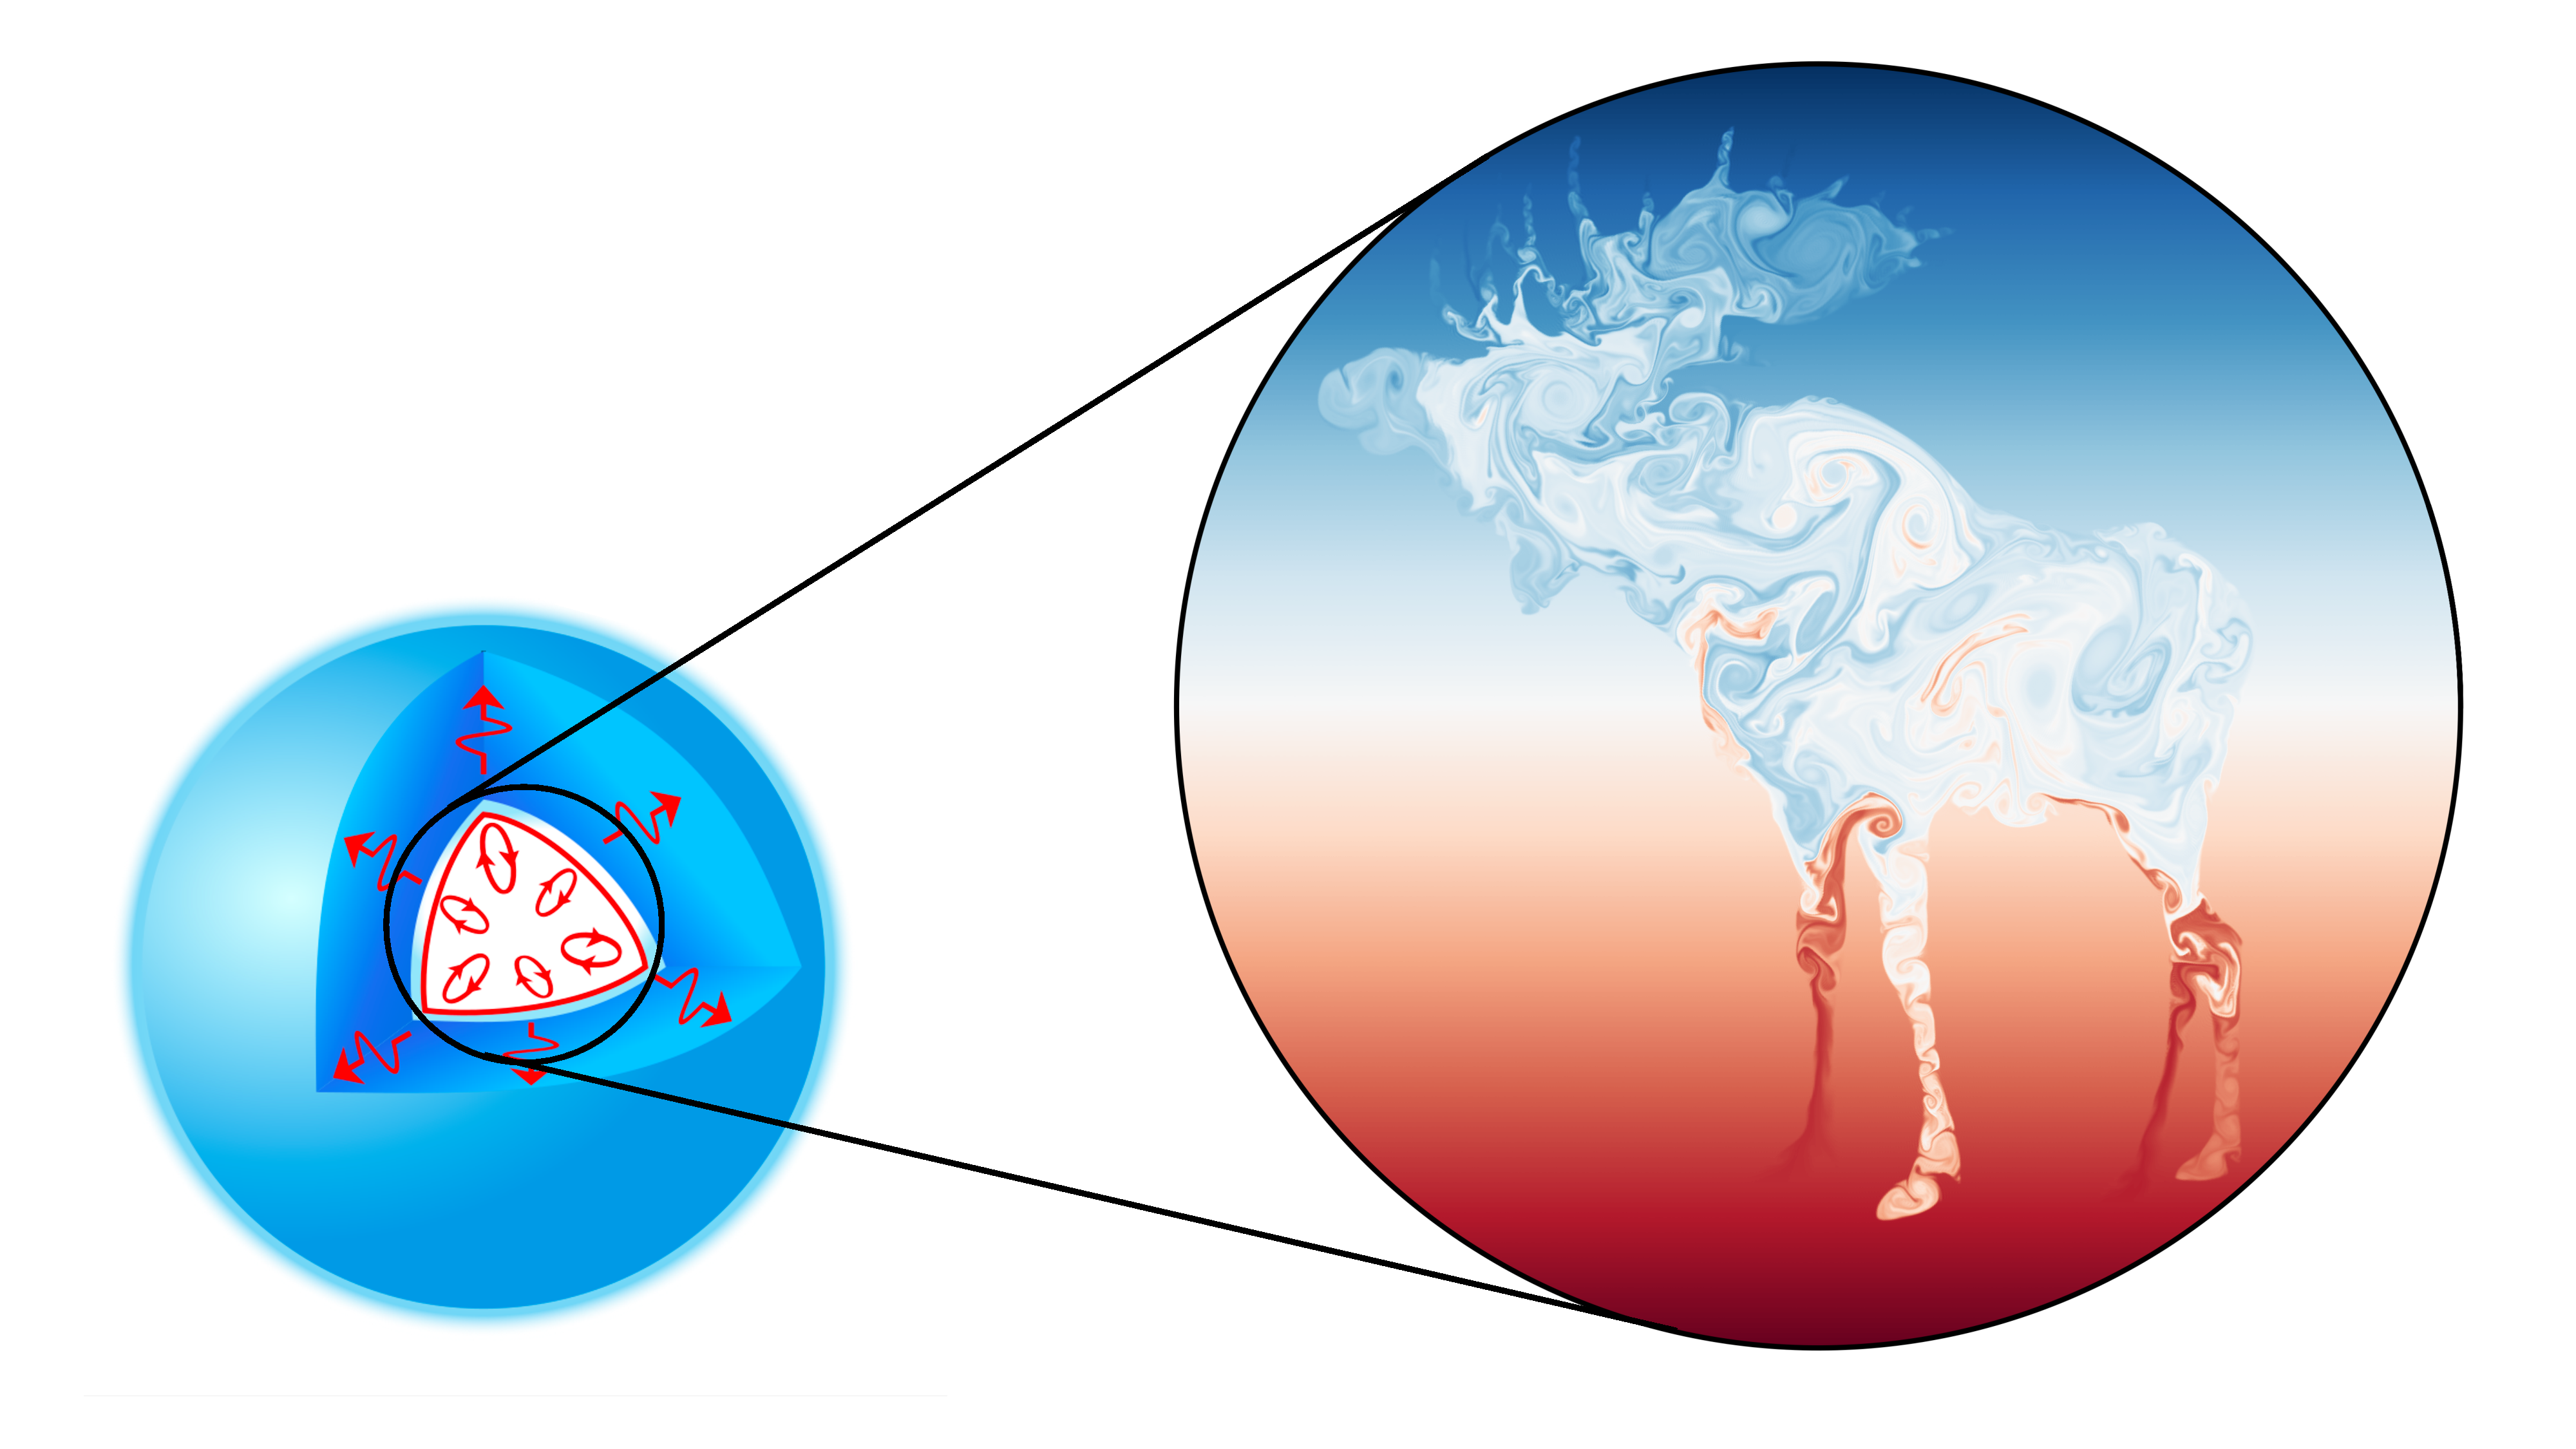
\includegraphics[width=\textwidth]{moosive_stars.pdf}
\caption{
    (Left) A diagram of a moosive star (source: \url{https://en.wikipedia.org/wiki/Stellar_structure}).
    (Right) The temperature field present in Moosinesq convection.
    We plot a circle around the core of the moosive star; we also plot some lines that lead to the circle around the Moosinesq convection simulation domain.
    This suggests that this convection is likely found within the core of these stars, but making this figure has increased our confusion as much as yours.
\label{fig:moosive_stars}
}
\end{figure*}




\section{Conclusions \& Discussion}
\label{sec:conclusions}

Future work: Elkman number, Mooselt number.

The methods developed in this work may suggest a pathway toward
unraveling the mysteries of other wildlife-related fluid phenomena,
such as the powerful and mysterious otter of \cite{Schwab2021}, also
known as the Papaloizou-Pringle Patronus.
Lessons learned from this and future work on the moosinesq approximation may also be of interest to those working in the yet-underexplored field of \textit{goosinesq} convection.

%The Boussinesq approximation is a commonly-used approximation in the field of fluid dynamics [liberal citations of authors' work here].
%It has [certain advantages] and [certain disadvantages], and is ultimately recognized for its great utility in [fluids jargon here].

However, the Boussinesq approximation must be abandoned in situations where compressibility is an important consideration.
This can occur in microbiology \citep{Ravetto2014}, and it has long been known that wildlife ecology is another such situation \citep[e.g.][]{Enright1963}.
Such studies have often focused on domains in which animal compressibility is more pronounced (i.e. deep-sea life).
However, motivated by a recent report of an unexpected occurrence of acute compression and deformation in a land-animal context \citep{Gudmannsson2018}---as well as a delightful linguistic coincidence---we present ground-breaking work on fundamental fluid dynamics in the context of the moose (\textit{Alces alces}), a domain which we dub the \textit{moosinesq approximation}.
This approximation is suitable for describing the active and dynamic inner lives and environments (both physical and mental; see \citealp{Gibson2015}) of the moose.

The moose is a large mammal indigenous to North America and Europe, which can have a mass of up to 550~kg and a height of up to 2~m \citep{CPWmoose}.
...
Our study is not the first time that moose have prompted significant scientific or technological development \citep[see, e.g.,][]{Handel2009}.

\subsection{Historical context}

The circumpolar distribution of Alces alces (moose) has led to multiple independent points of cultural connection to and subsequent efforts directed at harnessing the largest cervid with varying levels of success. 
Rock carvings in the Kalbak-Tash group, Altai Republic, Russia indicate that ab antuquo efforts to ride or cause moose to pull sleds have been documented and subsequently received comment since the Bronze Age and likely earlier \citep{useev_2014}.
In North America, European efforts to colonize Canada have been intermittently aided by the capture of wild individual moose more suited to traversing long distances in snow and over boggy ground than domestic alternatives leading to practical applications such as the use of a team of moose to deliver mail by Mr. W.R. Day \citep{archives_unleashed}.
The exploitation of this practicality was limited, obviously, by the size and temperament of the moose which after about the age of 3 days is entirely antagonistic towards humans \citep{sipko_etal_2019}.
A few spectacular exceptions of moose under harness has kept hope burning for a future with a less fraught relationship. 
The most noteworthy partnership is widely remembered through the efforts of Albert Vaillancourt of Chelmsford, Ontario who exhibited moose pulling a surrey during the intermissions of horse racing \citep{chisholm_2019}.
His pair of racing mooses named Moose and Silver clearly demonstrated the majesty and potential of this species \citep{landry_1941}.
 
This potential inspires the continuing quest for a fully domestic moose that is somewhat less likely to attack and kill humans. 
In Russia, moose domestication is the subject of investigations initiated by Prof. P. A. Manteifel who oversaw an effort to create moose nurseries across Russia for the purpose of creating a recognizably domestic animal from about 1934 through the present \citep{sipko_etal_2019}.
In an early, perhaps premature demonstration on December 1937, I.V. Stalin watched a military moose drill. 
He was, “particularly impressed by the moment when moose cavalry flew out of the forest, bristling with machine guns.” He did note that the moose were not yet trained to distinguish the Red Army soldiers from the White Finns \citep{pererva_2017}.


\begin{acknowledgments}
    We thank the Dedalus development team for creating an excellent tool that lets us create \sout{stupid} groundbreaking simulations like the one studied here.
    EHA is funded as a CIERA Postdoctoral fellow and would like to thank CIERA and Northwestern University. 
    This research was supported in part by the National Science Foundation under Grant No. PHY-1748958, and we acknowledge the hospitality of KITP during the Probes of Transport in Stars Program.
    The Flatiron Institute is supported by the Simons Foundation.
\end{acknowledgments}

\appendix

\section{Historical human-moose interactions}
\label{app:history}

The circumpolar distribution of Alces alces (moose) has led to multiple independent points of cultural connection to and subsequent efforts directed at harnessing the largest cervid with varying levels of success. 
Rock carvings in the Kalbak-Tash group, Altai Republic, Russia indicate that ab antuquo efforts to ride or cause moose to pull sleds have been documented and subsequently received comment since the Bronze Age and likely earlier \citep{useev_2014}.
In North America, European efforts to colonize Canada have been intermittently aided by the capture of wild individual moose more suited to traversing long distances in snow and over boggy ground than domestic alternatives leading to practical applications such as the use of a team of moose to deliver mail by Mr. W.R. Day \citep{archives_unleashed}.
The exploitation of this practicality was limited, obviously, by the size and temperament of the moose which after about the age of 3 days is entirely antagonistic towards humans \citep{sipko_etal_2019}.
A few spectacular exceptions of moose under harness has kept hope burning for a future with a less fraught relationship. 
The most noteworthy partnership is widely remembered through the efforts of Albert Vaillancourt of Chelmsford, Ontario who exhibited moose pulling a surrey during the intermissions of horse racing \citep{chisholm_2019}.
His pair of racing mooses named Moose and Silver clearly demonstrated the majesty and potential of this species \citep{landry_1941}.
 
This potential inspires the continuing quest for a fully domestic moose that is somewhat less likely to attack and kill humans. 
In Russia, moose domestication is the subject of investigations initiated by Prof. P. A. Manteifel who oversaw an effort to create moose nurseries across Russia for the purpose of creating a recognizably domestic animal from about 1934 through the present \citep{sipko_etal_2019}.
In an early, perhaps premature demonstration on December 1937, I.V. Stalin watched a military moose drill. 
He was, “particularly impressed by the moment when moose cavalry flew out of the forest, bristling with machine guns.” He did note that the moose were not yet trained to distinguish the Red Army soldiers from the White Finns \citep{pererva_2017}\footnote{Some internet sources believe that this was not truly said, but today is April 1, so it stands in our manuscript.}.


\section{Moose Mask Creation}
\label{app:mask}

The Moose is implemented using the volume penalization method described in e.g., \citet{hester_etal_2021}.
We first take an image of a majestic moose from the internet (Fig.~\ref{fig:methods}, left\footnote{Available online at \url{https://www.publicdomainpictures.net/en/view-image.php?image=317077&picture=moose}.}).
We convert this image into polar coordinates on the grid space representation of our basis function (Fig.~\ref{fig:methods, center}).

We then interpolate from pixel values into polar coordinates ($r$, $\phi$) sampled on the natural grid of our spectral bases (Fig.~\ref{fig:methods}, middle).
The resulting moose mask which is fed directly into our equations during timestepping is thus produced and shown in Fig.~\ref{fig:methods}, right.

We next compute a signed distance function $d_s$ at each pixel to determine how far that pixel is from the edge of the moose.
We convert that signed distance function (whose range is [-0.5, 0.5]) into a profile that varies smoothly from 0 to 1 over the moose boundaries, $\mathcal{M} = 0.5(1 - \mathrm{erf}(\pi^{1/2}d/\delta))$.



\section{Nondimensional Equations, Simulation Details \& Data Availability}
\label{app:nondim_equations}

All of the python scripts and ipython notebooks used to create the simulation in this paper and the figures in this paper are available online in a github repository (\url{https://github.com/evanhanders/moosinesq_convection}).


\newpage
\bibliographystyle{aasjournal}
\bibliography{biblio}
\end{document}
